
\chapter{OBSERVER}

E' un design pattern \underline{comportamentale} utilizzato per gestire le relazioni uno a molti quando lo stato di uno degli oggetti cambia e si richiede 
l'aggiornamento automatico di altri oggetti dipendenti.
\medskip

Classico esempio è quello di excel dove abbiamo una cella caratterizzata da una formula che fa riferimento a più celle "satellite" ed ogni volta che modifichiamo il
valore di questi satelliti, la cella caratterizzata dalla formula cambia di conseguenza.
\medskip

Questo pattern è basato sul concetto di un oggetto (\textbf{subject}) che tiene traccia dei suoi osservatori (\textbf{observers}).

Tutti gli observer vengono notificati ogni volta che il subject cambia il suo stato (è il subject che notifica e non sono gli osservatori che controllano ogni 
tot tempo).

A quel punto ogni observer può ispezionare lo stato del subject e aggiornare il proprio stato.

\medskip
\textbf{N.B.} Il subject non conosce quali observer lo osservano, lui si mantiene una lista di observer ma non conosce la loro implementazione concreta 
(\textbf{accoppiamento astratto} o abstract coupling).

Quando notifca, lui non sa a chi sta veramente notificando.
\medskip

Questo pattern favorisce la riduzione della dipendenza tra il soggetto e gli osservatori, permettendo di aggiungere o rimuovere osservatori senza modificare il 
soggetto stesso. 

Inoltre, favorisce un design flessibile e scalabile, permettendo di gestire in modo efficiente le relazioni tra gli oggetti in un sistema software.

\section{Struttura}

\begin{figure}[h]
    \centering
    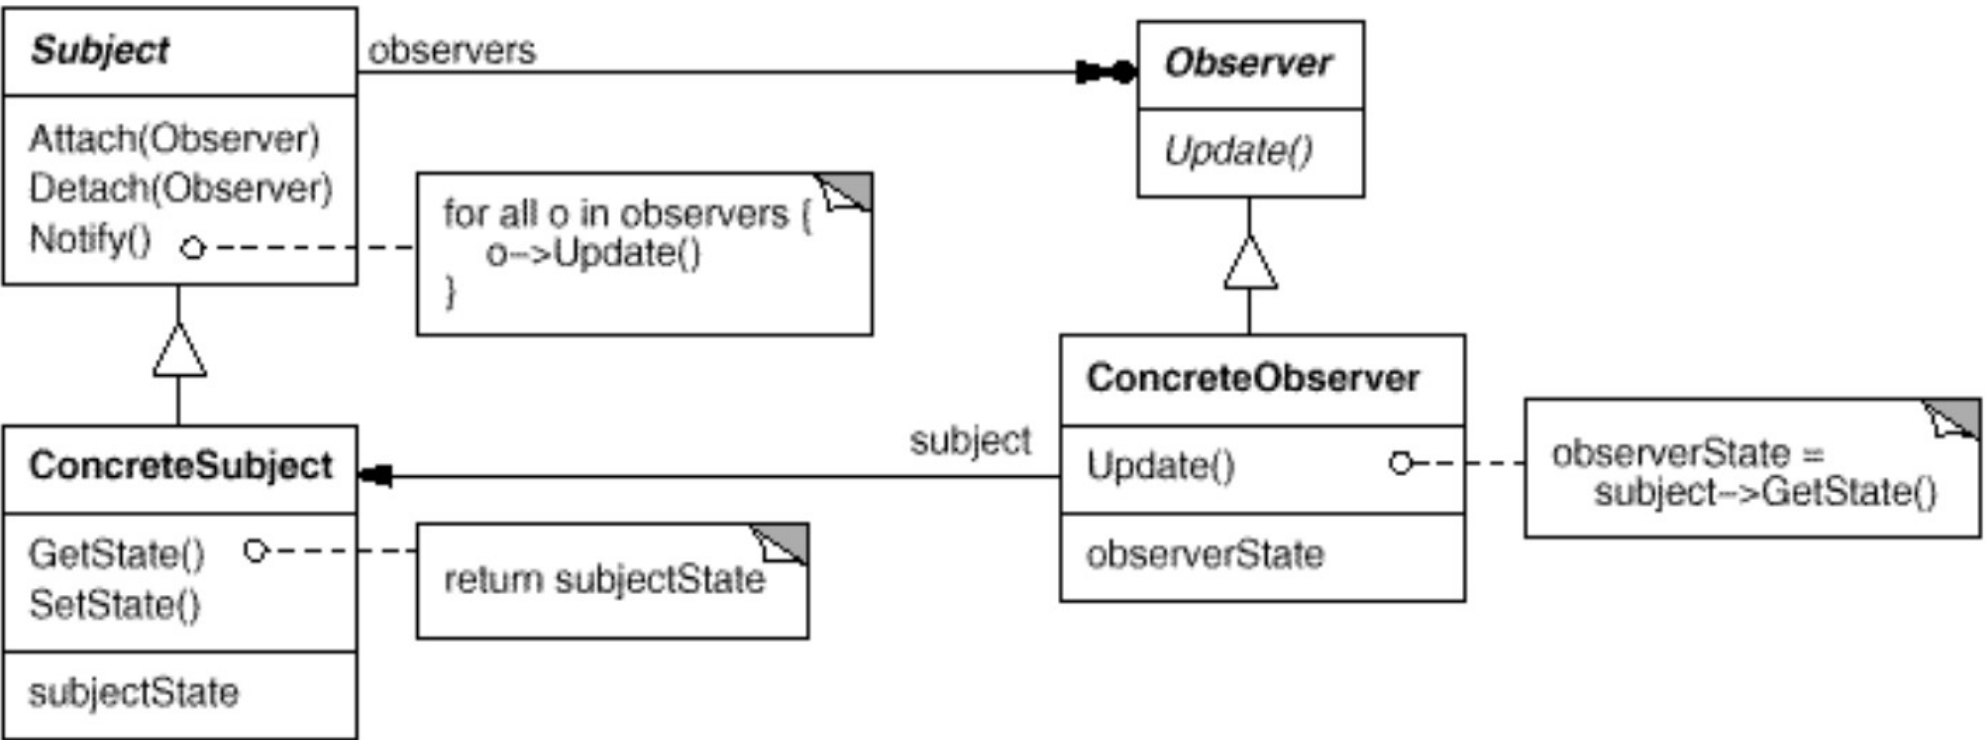
\includegraphics[width=0.5\linewidth]{../../immagini/observer_publishSubscribe/struttura_observer}
\end{figure}

\textbf{Subject} fornisce un'interfaccia per aggiungere, rimuovere e notificare gli Observer, ne conosce solamente l'interfaccia e può essere osservato da qualsiasi 
Observer.

\textbf{Observer} definisce l'interfaccia per gli oggetti che devono essere notificati riguardo il cambiamento del Subject.

\textbf{ConcreteSubject} mantiene uno stato da fornire ai ConcreteObserver.

\textbf{ConcreteObserver} ha un riferimento a ConcreteSubject ed un proprio stato che deve essere consistente al ConcreteSubject. 

\section{Interazione}

ConcreteSubject notifica i suoi osservatori quando avviene un cambiamento che potrebbe rendere lo stato degli Observer inconsistente col proprio.

Durante la notifica il ConcreteObserver può ispezionare il Subject per ottenere le informazioni per aggiornare il proprio stato, in modo da renderlo consistente con
quello del Subject.

\section{Conseguenze}

Observer non si riferisce a Subject ma è Subject che si riferisce agli Observer notificandoli.

ConcreteObserver ha un riferimento diretto a ConcreteSubject, mentre ConcreteSubject non lo ha, lo fa indirettamente chiamando il metodo di notifica ereditato da 
Subject.

Il Subject invia una notifica, in modalità broadcast a tutti i suoi Observer e spetterà all'Observer capire se la notifica è di suo interesse oppure no.

\section{Notifica}

Se la notifica parte dal Subject, allora i client non sono responsabili della notifica ma se il client cambia in sequenza più campi dello stesso Subject, allora 
avremo numerose notifiche consecutive (inefficienza).

Se la notifica viene chiamata dal client, ad esempio dopo vari cambiamenti chiama la notifica, è lui il responsabile della chiamata ma almeno si evitano le numerose 
notifche continue (sperando che il client si ricordi di chiamare la notifca).

\section{Svantaggio}

Il pattern è sincrono, ovvero, durante la notifica, aspetta che tutti i suoi Observer aggiornino il proprio stato.

Uno di questi Observer potrebbe essere maldestro, nel senso che ci mette troppo tempo, bloccando tutti gli altri, oppure maligno, magari lanciando un'eccezione.

\chapter{PUBLISH SUBSCRIBER}

Pattern basato su messaggi, abbiamo un Publisher che invia il messaggio ed un Subscriber che si sottoscrve ad un certo tipo di messaggio.

\section{Publish subscribe vs Observer}

I Publisher non inviano direttamente il messaggio ai Subscriber (mentre nel Observer è prorpio così) ma sono affidati ad un intermediario (\textbf{broker}) che si 
occupa di consegnare il messaggio al Subscriber appropriato (nell'Observer sono loro a decidere se è di loro interesse o meno).

Quindi Publisher e Subscriber sono completamente scorrelati (mentre nel Observer abbiamo una specie di accoppiamento astratto).

Questo pattern è asincrono (mentre l'altro è l'opposto), ovvero una volta che il Publisher consegna il messaggio al broker, lui continua a svolgere i propri compiti 
ed i mesaggi saranno consegnati, non subito, ai Subscriber appropriati (thread paralleli) ed è alla base dei sistemi ad evento (java swing) dove il messaggio è l'evento 
e i subscribe sono chiamati listener che si registrano e rimangono in ascolto di un determinato evento.

Questo pattern permette di avere un filtraggio dei messaggi, i subscriber dichiarano interesse per un certo tipo di messaggio e il broker si occuperà di consegnare ai 
subscriber solo i messaggi appropriati, invece, in Observer, spetta agli osservatori occuparsi manualmente del filtraggio.